\documentclass[10pt,UTF8]{book} %% ctexart

\title{\textbf{《操作系统》}实验报告}
\author{钱锋\thanks{Email: strik0r\_qf@mail.nwpu.edu.cn}}

\usepackage{ctex}
\usepackage{graphicx}
\usepackage[toc]{multitoc}
\usepackage{booktabs}
\usepackage{longtable}
\usepackage{amsthm, amssymb, amsmath, mathrsfs, mhchem}
\usepackage{tikz,circuitikz}
\usetikzlibrary{decorations.markings, angles, quotes}
\usetikzlibrary{shapes,arrows.meta,positioning}
\usepackage{tikz-cd}
\usepackage{pgfplots}
\usepackage{tikz-3dplot}
\usepackage{extpfeil}
\usepackage{diagbox}
\usepackage{float}
\usepackage{hyperref}
\hypersetup{hidelinks,
    colorlinks = true,
    allcolors = black,
    pdfstartview = Fit,
    breaklinks = true}
\usepackage{caption}
\usepackage{enumitem}
\usepackage{siunitx}
\usepackage{subcaption}
\usepackage{tasks}
\usepackage{lipsum} % For dummy text

\usepackage{titlesec} % 定义标题样式

% 设置 chapter 标题样式
\titleformat{\chapter}[hang]{\centering\heiti\Large\bfseries}{实验\,\thechapter}{1em}{}

% 定义 section 标题格式
\titleformat{\section}[hang]{\heiti\centering\large\bfseries}{\thesection}{1em}{}

% 定义 subsection 标题格式
\titleformat{\subsection}[hang]{\heiti\bfseries}{\textbf{\thesubsection}}{1em}{}

% 定义 subsubsection 标题格式
\setcounter{secnumdepth}{3}
\renewcommand\thesubsubsection{\arabic{subsubsection}.}
\titleformat{\subsubsection}[hang]{\kaishu}{\quad\quad\thesubsubsection\,\,}{0em}{}

\usepackage{titletoc}

\input{../_mdframed_settings.tex}

% 页面设置
\input{../_geometry_setteings.tex}

% 页眉页脚的设置
\input{../_fancyhdr_settings.tex}

% 设置代码块
\input{../_listings_settings.tex}

\usepackage{smartdiagram} % 表格对角线
\everymath{\displaystyle}
\usepackage{tasks}

\begin{document}
\input{../_theoremstyles.tex}
\pagestyle{empty}
% 使用 IEEE 样式
\ctikzset{logic ports=ieee}

\begin{titlepage}
    \thispagestyle{empty}
    \centering
        \vspace*{2cm}
        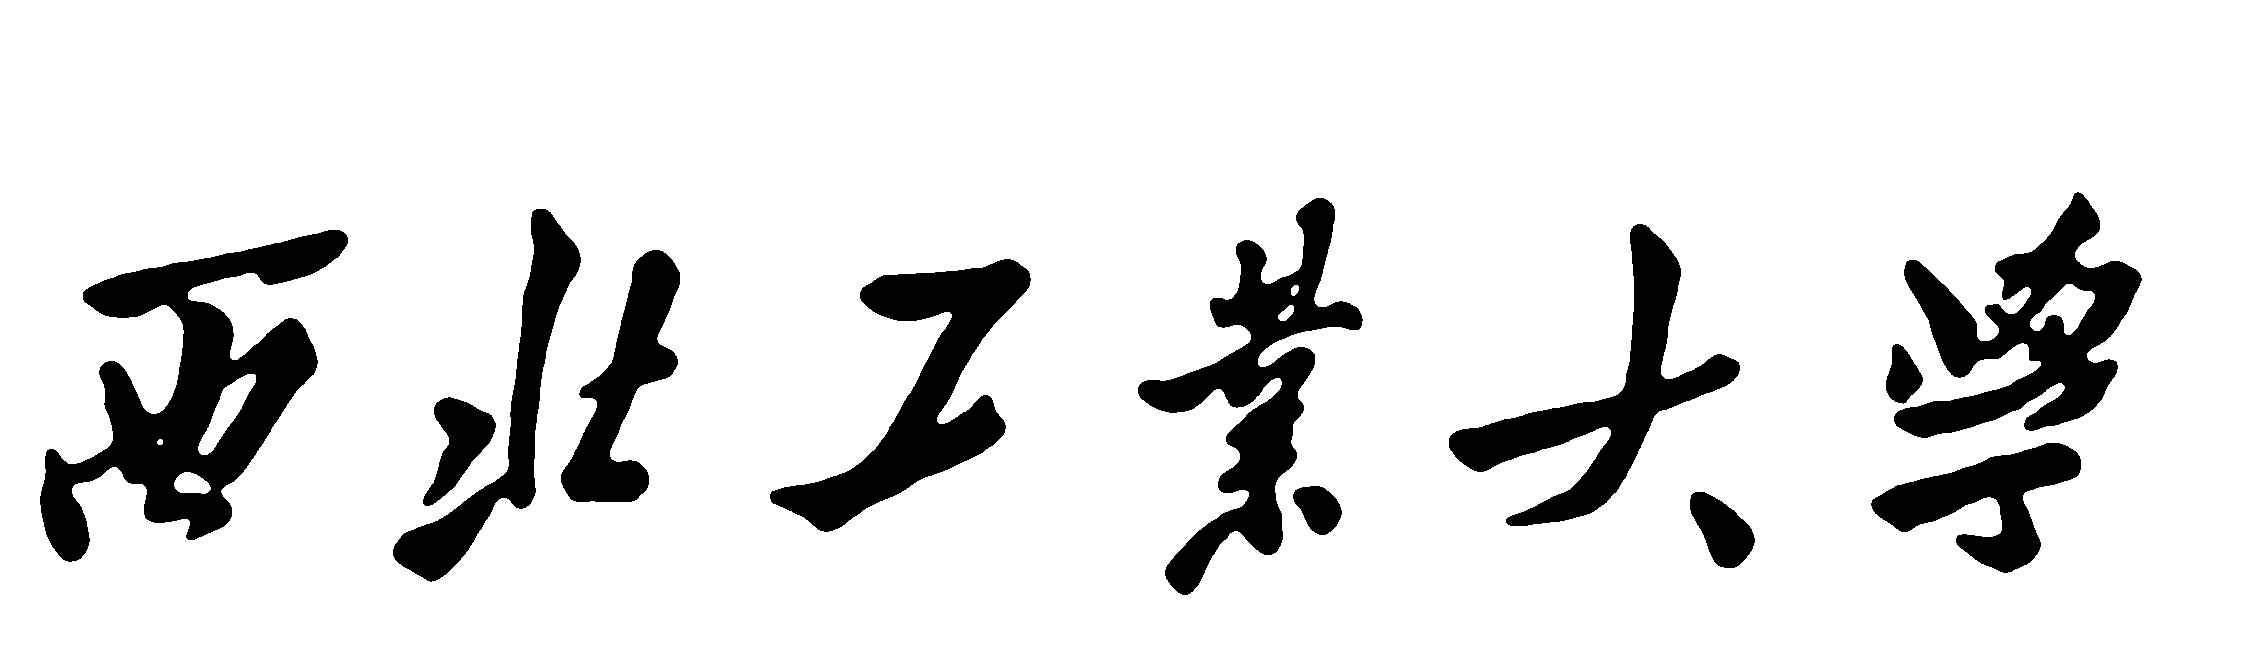
\includegraphics[width=0.5\textwidth]{../npu_2.png}\par
        \vspace{1em}
        
\includegraphics[width=0.5\textwidth]{../npu_1.png}\par
    \vspace{2em}
        \begin{center}
            \Huge \heiti \textbf{《操作系统》实验报告}

            Operating Systems: Experiment Report
        \end{center}
        \vspace{3cm}
        \begin{center}
        \songti
        \renewcommand\arraystretch{1.5}
	\begin{tabular}{p{2cm} c c}
    {姓\,\,\,\,\,\,\,\,\,\,\,\,名:} & \multicolumn{2}{c}{钱 \quad\quad 锋}\\
    \cline{2-3}
    % {编\,\,\,\,\,\,\,\,\,\,\,\,号:} & \multicolumn{2}{c}{13} \\
    % \cline{2-3}
    {班\,\,\,\,\,\,\,\,\,\,\,\,级:} & \multicolumn{2}{c}{14012203} \\
    \cline{2-3}
    {学\,\,\,\,\,\,\,\,\,\,\,\,号:} & \multicolumn{2}{c}{2022303324}\\
    \cline{2-3}
    {邮\,\,\,\,\,\,\,\,\,\,\,\,箱:} & \multicolumn{2}{c}{strik0r.qf@gmail.com}\\
    \cline{2-3}
    {日\,\,\,\,\,\,\,\,\,\,\,\,期:} & \multicolumn{2}{c}{\today}\\
    \cline{2-3}
	\end{tabular}
    \end{center}
\end{titlepage}
\cleardoublepage
\maketitle

\frontmatter
\newpage
\pagestyle{plain}
\makeatother

% \input{丛书前言.tex}

% \chapter{课程概述}
% \thispagestyle{empty}

% \newpage
% \thispagestyle{empty}

% 设置目录页的页码格式
\pagenumbering{roman} % 切换回罗马数字页码
\addtocontents{toc}{\protect\thispagestyle{empty}}
\pagestyle{plain}
{\tableofcontents}
\newpage
\thispagestyle{empty}
\cleardoublepage % 确保正文从奇数页开始


% 设置章节标题页的页眉和页脚为空白页样式
\makeatletter
\let\ps@plain\ps@empty
\makeatother

\mainmatter
\renewcommand{\chaptermark}[1]{\markboth{实验 \thechapter\hspace{1em} #1}{}} % 在章节标题前添加 "Chapter x: "
\renewcommand{\sectionmark}[1]{\markright{\thesection \, #1}} % 如果需要定义\rightmark,可以使用这行代码

\chapter{openEuler 操作系统安装与内核编译}

\input{../_appendix.tex}

\onecolumn
\begin{thebibliography}{1}
    \addcontentsline{toc}{chapter}{参考文献}
    \bibitem{汤小丹}
    汤小丹等. 计算机操作系统: 慕课版 [M]. 北京: 人民邮电出版社, 2021.
    \bibitem{王道操作系统}
    王道论坛组. 2024 年操作系统考研复习指导 [M]. 北京: 电子工业出版社, 2022.
    \bibitem{实验指导}
    王红玲, 储晓敏. 计算机操作系统实验指导: Linux 版: 附微课视频 [M].
    北京: 人民邮电出版社, 2021.
\end{thebibliography}

\newpage
\thispagestyle{empty}
\vspace*{4cm}
\begin{center}
    \includegraphics*[width=\textwidth]{../pic/Keynote素材库.001.jpeg}
    \large
    公诚勇毅 \quad 永矢毋忘

    中华灿烂 \quad 工大无疆
\end{center}
\vspace*{5cm}
\begin{center}
    \small
    本文档由\textbf{钱锋}编写, 钱锋保留一切权利.

    文档中出现的部分素材来源于网络, 笔者承诺这些素材仅供学习交流之用, 
    它们的原作者保留一切权利.

    2023 年 \quad 西北工业大学 \quad 中国西安 
\end{center}

\end{document}